\section{Einführung in die Programmierung grafischer Benutzeroberflächen mit JavaFX}


Eine grafische Benutzeroberfläche besteht i.d.R aus \textbf{Controls} und \textbf{Widgets}: \textbf{Buttons}, \textbf{Labels}, \textbf{Input-Elemente} (Textfelder)...\\

\noindent
Anordnung dieser Elemente wird mit Hilfe von Layouts realisiert, die verschachtelt sein können.\\

\noindent
Strukturen dieser Anordnungen können als Baumstrukturen verstanden werden, mit dem ``Fenster`` als Wurzel.\\

\noindent
In JavaFX wird ein Fenster als \code{Stage} bezeichnet.\\

\noindent
Das erste Fenster einer Anwendung muss man nicht selbst erstellen, sondern existiert bereits und wird zur Verfügung gestellt.\\

\noindent
Eine \code{Stage} beinhaltet keine UI Controls, sondern eine \code{Scene}, der dann weitere Elemente (i.d.R. zunächst ein ``Container``) hinzugefügt werden.\\

\noindent
Üblicherweise erzeugt man eine JavaFX-Anwendung, indem man von \begin{center}\code{javafx.application.Application}\end{center} erbt, die \code{start()}-Methode überschreibt und darin die der Methode übergebenen \code{Stage} eine \code{Scene} zuweist und dann mittels \code{show()} sichtbar macht:

\begin{minted}[mathescape,
    linenos,
    numbersep=5pt,
    gobble=2,
    frame=lines,
    framesep=2mm]{java}
    public class JavaFxDemo extends Application {

        public void start(Stage primaryStage) {
            Hbox root = new Hbox();
            hbox.getChildren().add(...);
            ...
            Scene s = new Scene(hbox);
            ...
            primaryStage.setScene(scene);
            primaryStage.show();
        }

        public static void main(String[] args) {
            launch(args);
        }

    }
\end{minted}

\begin{tcolorbox}[enlarge top by=0.5cm,enlarge bottom by=0.5cm]
    Die Methode \code{launch} ist blockierend, aus ihr kehrt man erst zurück, wenn die \textbf{PrimaryStage} geschlossen wurde.
\end{tcolorbox}

\noindent
Elemente werden Containern nicht mittels ``add`` o.ä. hinzugefügt, sondern man ruft die Liste der Kindelemente über \code{getChildren()} ab und fügt dieser dann die Kindelemente hinzu.\\

\noindent
Gibt man bei der \code{Scene} keine Größenangabe an, versucht JavaFX, die Fenstergröße so anzupassen, dass die Scene dargestellt werden kann.

\subsection{Ereignisbehandlung}

Nutzeraktionen werden ``Ereignisse`` genannt; die Behandlung solcher Ereignisse über Programmcode wird \textbf{Ereignisbehandlung} genannt.\\

\noindent
So kann zum Beispiel ein \code{javafx.scene.control.Button} auf Mausereignisse reagieren, indem man

\begin{center}\code{+setOnAction(value: EventHandler<ActionEvent>):void}\end{center}

implementiert. \code{value} enthält dann die Ereignisinformationen.

\begin{tcolorbox}[enlarge top by=0.5cm,enlarge bottom by=0.5cm]
    Bei dem Typ des Parameters für die \code{setOnAction()}-Methode handelt es sich um das \textit{Functional Interface}
     \begin{center}
     \code{java.fx.event.EventHandler<T extends Event>}
     \end{center}
    mit der abstrakten Methode \code{handle(T event)}\footnote{
        Interface EventHandler<T extends Event>: \url{https://docs.oracle.com/javase/8/javafx/api/javafx/event/EventHandler.html#handle-T-} - abgerufen 28.01.2024
    }
\end{tcolorbox}

\noindent
\textbf{Ereignisbehandlungen} werden i.d.R. durch \textbf{Upcalls} ausgelöst: Die JavaFX-Bibliothek enthält die Logik zur Verarbeitung nativer Ereignisse und ruft den Code des Entwicklers auf, die wiederum über \textbf{Downcalls} Logik der Bibliothek nutzen kann.

\begin{figure}
    \centering
    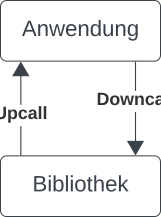
\includegraphics[scale=0.5]{chapters/fopt3/img/javafx/downcallupcall}
    \caption{Downcalls und Upcalls zwischen Anwendung und Bibliothek. (Quelle: eigene)}
    \label{fig:downcallupcall}
\end{figure}

\section{Properties, Bindings und JavaFX-Collections}

\subsection{Properties}

Das allgemeine Prinzip der Ereignisbehandlung basiert auf dem Entwurfsmuster \textbf{Observer}: $\rightarrow$ es gibt \textbf{beobachtbare Objekte} und \textbf{Beobachter}.\\

\noindent
\textbf{Beobachter} melden sich bei \textbf{beobachtbaren Objekten} an und werden über Zustandsänderungen benachrichtigt.\\

\noindent
Die Benachrichtigung erfolgt über Schnittstellenmethoden, die die Beobachter implementieren; die Schnittstellen sind die Typen der Parameter, die ein beobachtbares Objekt bei der Registrierung eines Beobachters berücksichtigen - es können also nur solche Objekte als Beobachter angemeldet werden, deren Klasse die Schnittstelle implementiert.\\

\noindent
\textbf{Properties} in JavaFX sind Klassen, die dieses Prinzip implementieren, und sind im Allgemeinen \textbf{beobachtbare Objekte}, bspw.

\begin{itemize}
    \item \code{SimpleIntegerProperty}
    \item \code{SimpleBooleanProperty}
    \item \code{SimpleObjectProperty<T>}
    \item {...}
\end{itemize}


\noindent
Spezielle Varianten der Properties sind die \code{ReadOnlyProperty}s - diese können von \code{ReadOnlyWrapper}n zur Verfügung gestellt machen, um beobachtbare Properties öffentlich zu machen, aber deren Zustandsänderung von außen zu untersagen, wie folgendes Beispiel demonstriert:

\begin{minted}[mathescape,
    linenos,
    numbersep=5pt,
    gobble=2,
    frame=lines,
    framesep=2mm]{java}]
    public class Foo {

        private ReadOnlyIntegerWrapper value;

        ...

        public ReadOnlyInteger value() {
            return value.getReadOnlyProperty();
        }

        public void setValue(int v) {
            value.set(v);
        }

    }
\end{minted}\\

\subsection{Bindings}

Properties können miteinander gekoppelt werden, um gegenseitige Zustandsänderungen zu bewirken.\\

\noindent
Die Kopplung (das \textbf{Binding}) kann \textbf{unidirektional} oder \textbf{bidirektional} erfolgen.\\

\noindent
Bei \textbf{unidirektionalem} Binding bewirkt die Änderung des Wertes einer Property die Änderung des Wetes der anderen Property, aber nur in eine Richtung.\\
Wird versucht, über die andere Richtung eine Wertzuweisung durchzuführen, wird eine Exception geworfen.\\
Eine JavaFX-Property kann über \code{right.bind(left)} gekoppelt werden (lies: ``binde right an left``).\\

\noindent
Ein \textbf{bidirektionales} Binding bewirkt die Änderung der Properties in beide Richtungen, allerdings muss hier die Methode \begin{center}\code{+bindBidirectional(other: Property<T>):void}\end{center} genutzt werden: \code{right.bindBidirectional(left)} (bzw. \code{left.bindBidirectional(right)}).


\begin{figure}
    \centering
    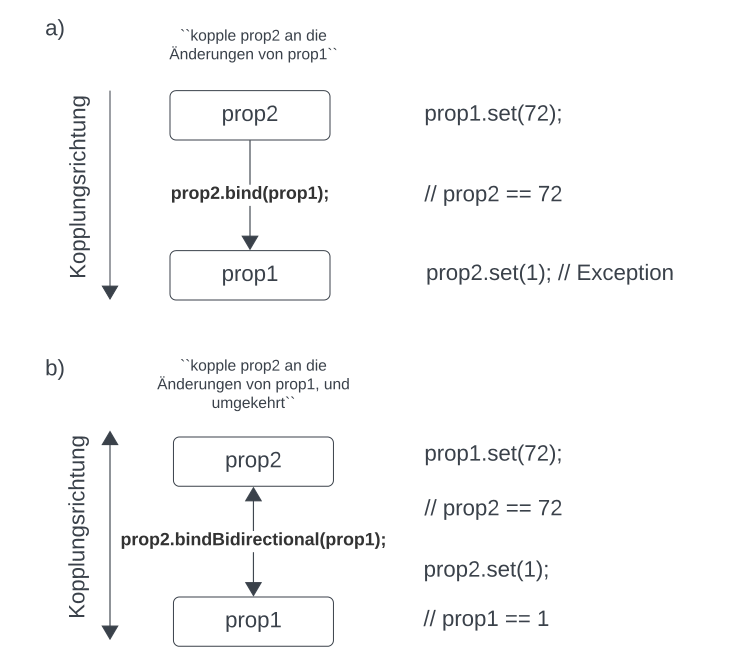
\includegraphics[scale=0.5]{chapters/fopt3/img/javafx/binding}
    \caption{Unidirektionales (a) und Bidirektionales (b) Binding in JavaFX. Die Properties sind vom Typ SimpleIntegerProperty. (Quelle: eigene)}
    \label{fig:binding}
\end{figure}

\subsection{JavaFX-Collections}

\textbf{Collections} sind in JavaFX Schnittstellen und Implementierungen, um Daten über einen ``Behälter`` zu verwalten (Listen, Mengen, Hash-Tabellen...).\\

\noindent
Collections in JavaFX erweitern die Collections von Java\footnote{
    ``Java collections framework``: \url{https://en.wikipedia.org/wiki/Java_collections_framework}: abgerufen 29.01.2024

}, um die Property-Charakteristik, sie sind also genauso \textit{observable}, wie bspw.: \code{ObservableList}, \code{ObservableMap}, \code{ObservableSet}.\\

\noindent
In der Regel werden diese Collections von den Container-Elementen verwendet, die ein bestimmtes \textbf{Layout} realisieren.\\

\noindent
$\rightarrow$ für den Zugriff auf die Kindelemente eines Containers in JavaFX ruft man i.d.R. \code{getChildren} auf; der Rückgabewert ist die beobachtbare Liste.

\begin{figure}
    \centering
    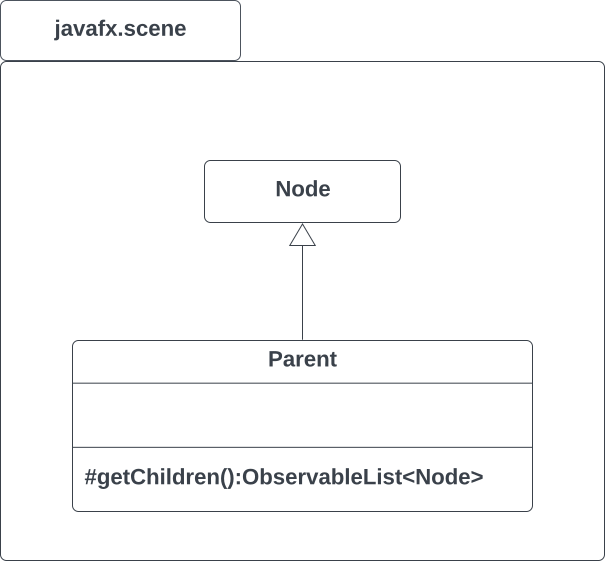
\includegraphics[scale=0.5]{chapters/fopt3/img/javafx/nodeparent}
    \caption{Parent ist in JavaFX eine Container-Klasse. getChildren() liefert eine beobachtbare Liste mit Kindelementen zurück. (Quelle: eigene)}
    \label{fig:nodeparent}
\end{figure}

\section{Elemente von JavaFX}

Die grafische Benutzeroberfläche besitzt eine baumartige Struktur.\\

\noindent
Elemente die Nachfolger in diesem Baum sind, sind \textbf{Container-Elemente}, die ein bestimmtes \textbf{Layout} realisieren für die darin enthaltenen Elemente.\\

\noindent
Elemente, die keinen Nachfolger besitzen, können unter dem Begriff \textbf{Interaktionselemente} zusammengefaßt werden (\code{Label}s, \code{Button}s, ...).

\subsection{Container}

\code{Node} ist die Basisklasse für Container und Interaktionselemente.\\

\noindent
\code{Pane} ist ein Kind von \code{Parent} und die Basisklasse für Container-Klassen.

\begin{figure}
    \centering
    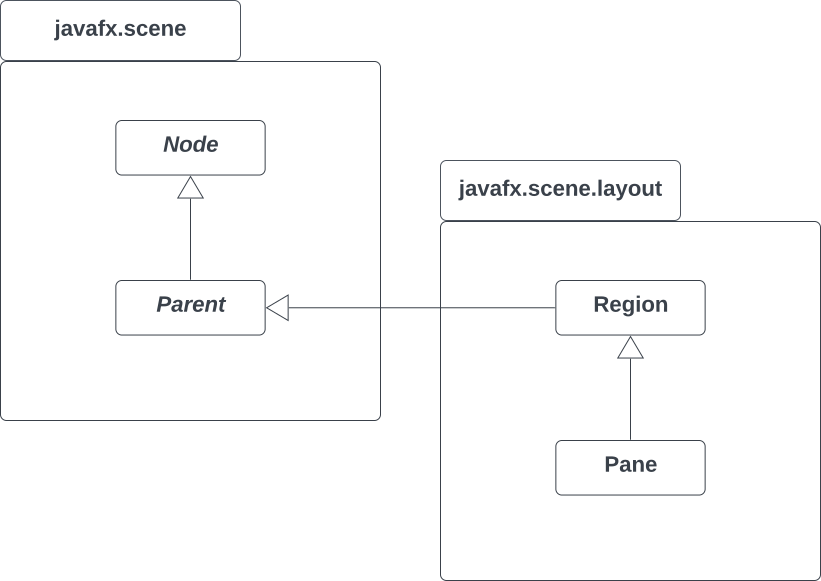
\includegraphics[scale=0.5]{chapters/fopt3/img/javafx/pane}
    \caption{Vererbungshierarchie der Container-Klasse Pane. (Quelle: eigene)}
    \label{fig:pane}
\end{figure}

\noindent
\code{Pane} selber realisiert kein Layout, Kindelemente werden absolut positioniert.\\

\noindent
Unterklassen von \code{Pane} hingegen realisieren verschiedene Layouts, bspw.

\begin{itemize}
    \item \code{VBox}
    \item \code{HBox}
    \item \code{FlowPane}
    \item \code{BorderPane}
    \item \code{StackPane}
    \item \code{TilePane}
    \item \code{GridPane}
    \item \code{AnchorPane}
\end{itemize}


\subsection{Interaktionselemente}

Interaktionselemente haben wie die Container-Klassen \code{Node} als Basisklasse.\\

\noindent
Die Klasse \code{Control} ist (über mehrere Klassen) von \code{Node} abgeleitet und (abstrakte) Basisklasse aller Interaktionselemente.

\begin{figure}
    \centering
    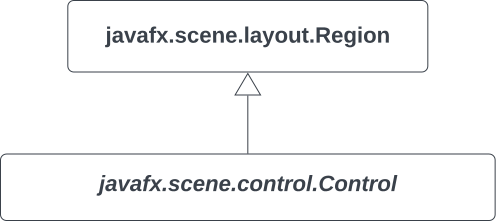
\includegraphics[scale=0.5]{chapters/fopt3/img/javafx/control}
    \caption{Die Klasse Control ist direkt von Region abgeleitet. (Quelle: eigene)}
    \label{fig:control}
\end{figure}



\noindent
Wichtige Interaktionslemente sind bspw. die von der abstrakten Klasse \code{Labeled} sogenannten \textbf{Command Buttons} und \textbf{Choice Buttons}.\\
Zu den Choice Buttons gehören bspw. \code{CheckBox}, \code{ToggleButton}, \code{RadioButton}.\\
Zu den Command Buttons gehören u.a. \code{Button} und \code{Hyperlink}.\\

\noindent
Eine \code{CheckBox} kann in JavaFX drei Zustände besitzen: \code{true}, \code{false}, \code{undefined} (steuerbar über \code{setAllowIndeterminate()}):

\blockquote[{Class CheckBox: \url{https://docs.oracle.com/javase/8/javafx/api/javafx/scene/control/CheckBox.html} - abgerufen 29.01.2024}]{
    A tri-state selection Control typically skinned as a box with a checkmark or tick mark when checked. A CheckBox control can be in one of three states:
    \begin{itemize}
        \item checked: indeterminate == false, checked == true
        \item unchecked: indeterminate == false, checked == false
        \item undefined: indeterminate == true
    \end{itemize}
}

\noindent
\code{ToggleButton}s und \code{RadioButton}s sind einander ähnlich, sie können selektiert und deselektiert werden.


\begin{figure}
    \centering
    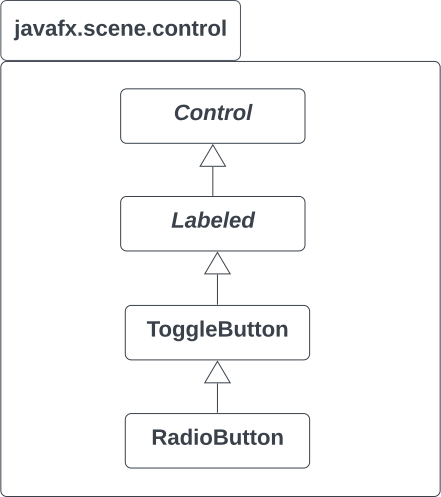
\includegraphics[scale=0.5]{chapters/fopt3/img/javafx/radiobutton}
    \caption{Die Klasse RadioButton im Package javafx.scene.control. (Quelle: eigene)}
    \label{fig:radiobutton}
\end{figure}

\noindent
\code{ToggleGroup} fasst Objekte dieser Klasse zusammen und erlaubt, dass höchstens ein Element dieser Gruppe selektiert sein kann.\\

\noindent
Darüber hinaus existieren Auswahlelemente wie \code{ChoiceBox}, \code{ComboBox}, \code{ListView}, \code{DatePicker}, \code{ColorPicker}, \code{FileChooser}.\\

\noindent
\code{ComboBox} ist ähnlich \code{ChoiceBox}, aber bietet mehr Funktionalität: So besitzt die Klasse Typparameter, der dem Typen der enthaltenen Elemente entspricht.\\
Änderungen der Auswahl erfährt man über einen \code{ChangeListener}\footnote{
    Interface ChangeListener<T>: \url{https://docs.oracle.com/javase/8/javafx/api/javafx/beans/value/ChangeListener.html} - abgerufen 29.01.2024
}, den man für den Rückgabewert von \code{valueProperty()}\footnote{
Der Rückgabewert ist \textit{ObjectProperty<T>}; die Klasse leitet von \textit{ReadOnlyObjectProperty<T>} ab.
} konfiguriert:

\begin{minted}[mathescape,
    linenos,
    numbersep=5pt,
    gobble=2,
    frame=lines,
    framesep=2mm]{java}
    ComboBox<String> cb = new ComboBox();
    cb.getItems().add("one");
    cb.getItems().add("two");
    cb.getItems().add("three");

    cb.valueProperty().addListener(
        (ObservableProperty<? extends String> ov,
        String oldValue,
        String newValue) -> {
            System.out.println(oldValue + "; " + newValue)
        }
    );
\end{minted}\\

\noindent
Eine \code{ComboBox} nutzt intern eine \code{ListView} zur Anzeige der Inhalte. \code{ListView} erlaubt sowohl Einfach- als auch Mehrfachauswahl.\\

\noindent
Texteingabeelemente wie \code{TextField}, \code{TextArea} sind von der abstrakten Basisklasse \code{TextInputControl} abgeleitet.\\

\noindent
\code{TextField} erlaubt mittels \code{setOnAction()} die Registrierung eines \code{EventHandler<ActionEvent>}.\\
Das Ereignis wird bspw. beim Betätigen der \textit{Return}-Taste ausgelöst:\\


\begin{minted}[mathescape,
    linenos,
    numbersep=5pt,
    gobble=2,
    frame=lines,
    framesep=2mm]{java}
    TextField f = new TextField();
    f.setOnAction((ActionEvent e) -> System.out.println(e));
\end{minted}\\

\noindent
\textbf{Numerische Werte} können anhand eines \code{Slider}s eingegeben werden.\\
\code{Slider} erlauben die Konfiguration von minimalen und maximalen Werten.\\
Der aktuelle Wert wird über eine \code{DoubleProperty} repräsentiert und kann über \code{valueProperty()} abgefragt werden.\\

\noindent
Weitere Interaktionselemente sind \code{ProgressBar}, \code{ProgressIndicator}, \code{TreeView}, \code{TableView}, \code{TreeTableView}.


\subsection{Grafikprogrammierung}

Unter \textbf{Grafikprogrammierung} versteht man das Zeichnen verschiedener Formen in ein Fenster.\\

\noindent
In JavaFX ist das realisiert durch Objekte verschiedener Klassen, die aus \code{Shape} abgeleitet sind.\\

\noindent
Die Basisklasse für Farben und Gradienten ist \code{Paint}.\\

\noindent
Es gibt verschiedene vordefinierte Konstanten für Farben, wie z.B. \code{Color.BLACK}, \code{Color.GREEN} usw.\\

\noindent
Eine \code{Shape} hat je eine \code{ObjectProperty<Paint>} für \textit{Linienfarbe} und \textit{Füllfarbe}, sowie eine \code{Double}-Property für die Liniendicke.\\

\noindent
Aus \code{Shape} abgeleitet sind bspw.

\begin{itemize}
    \item \code{Line}
    \item \code{Rectangle}
    \item \code{Circle}
    \item \code{Ellipse}
    \item \code{Polyline}
    \item \code{Polygon}
    \item \code{Arc}
    \item \code{QuadCurve}
    \item \code{CubicCurve}
    \item \code{Text}
    \item ...
\end{itemize}

\noindent
\textbf{Koordinaten} verlaufen in JavaFX i. A.

\begin{itemize}
    \item $x$: links $\rightarrow$ rechts
    \item $y$: oben $\rightarrow$ unten
\end{itemize}


\noindent
Bereits die Basisklasse \code{Node} stellt Funktionen zur Ereignisbehandlung von Mausereignissen zur Verfügung:

\begin{itemize}
    \item \code{setOnMousePressed()}
    \item \code{setOnMouseReleased()}
    \item \code{setOnMouseMoved()}
    \item ...
\end{itemize}

\noindent
Der Parametertyp für diese Ereignisbehandlung ist wie bei \code{setOnAction()} ein \code{EventHandler}, dessen generischer Typ auf \code{MouseEvent} festgelegt ist\footnote{
    oder einer Unterklasse davon, bspw. \textit{MouseDragEvent}
}.\\

\noindent
Zur Ereignisbehandlung von \textbf{click-Events} wird i.d.R. mithilfe eines \code{ActionListeners} reagiert, da solch ein Interaktionsereignis \uunderline{eine höhere Abstraktionsebene darstellt}, z.B. wird ein Button auch aktiviert, wenn er den Fokus hat und die \textbf{Enter-Taste} gedrückt wird:  Action-Ereignis $\rightarrow$ aktivieren eines Elements (vgl.~\cite[220]{Oec22}).


